%
% request format design
%

\documentclass[12pt]{article} % FORMAT CHANGE
\usepackage[dvips]{graphicx}
\usepackage{times}

\graphicspath{{./}{figs/}} 

%
% GET THE MARGINS RIGHT, THE UGLY WAY
%
% \topmargin 0.2in
% \textwidth 6.5in
% \textheight 8.75in
% \columnsep 0.25in
% \oddsidemargin 0.0in
% \evensidemargin 0.0in
% \headsep 0.0in
% \headheight 0.0in

\pagestyle{plain}

\addtolength{\hoffset}{-2cm}
\addtolength{\textwidth}{4cm}

\addtolength{\voffset}{-1.5cm}
\addtolength{\textheight}{3cm}

\setlength{\parindent}{0pt}
\setlength{\parskip}{12pt}

\title{PVFS2 MPI Based Requests\\ Design Notes}
\author{PVFS Development Team}
\date{march 2002}

\begin{document}

\maketitle

\section{PVFS Requests}

PVFS user programs can construct a data structure that represents a
specifc set of non-contiguous data that is to be read from or written to
a PVFS file.  The PVFS library includes a set of routines for creating
these structures in a controlled manner.  These routines produce an
opaque type the PVFS\_Request which is actually a pointer to an internal
structure, the PINT\_Request.

\begin{verbatim}
typedef struct PINT_Request *PVFS_Request; /* user type for requests */

int PVFS_Request_contiguous(int count, PVFS_Request oldreq,
            PVFS_Request *newreq);

int PVFS_Request_vector(int count, int blocklength, int stride,
            PVFS_Request oldreq, PVFS_Request *newreq);

int PVFS_Request_hvector(int count, int blocklength, int64_t stride,
            PVFS_Request oldreq, PVFS_Request *newreq);

int PVFS_Request_indexed(int count, int *blocklengths,
            int *displacements, PVFS_Request oldreq, PVFS_Request *newreq);

int PVFS_Request_hindexed(int count, int *blocklengths, int64_t *displacements,
            PVFS_Request oldreq, PVFS_Request *newreq);

int PVFS_Request_struct(int count, int *blocklengths, int64_t *displacements,
            PVFS_Request *oldreqs, PVFS_Request *newreq);

int PVFS_Address(void* location, int64_t *address);

int PVFS_Request_extent(PVFS_Request request, int64_t *extent);

int PVFS_Request_size(PVFS_Request request, int *size);

int PVFS_Request_lb(PVFS_Request request, int64_t* displacement);

int PVFS_Request_ub(PVFS_Request request, int64_t* displacement);
\end{verbatim}

These routines are based directly on the MPI datatype constructor routines
of similar name and have the same semantics.

\section{Request Data Structures}

The PINT\_Request is designed to represent any data layout that can
be specified using MPI's MPI\_Datatype constructors.  The
PINT\_Request\_state is a structure that indicates how much of a request
has actually been processed.  Using these structures it is possible to
process part of a PVFS request, stop, and then resume processing at a
later time when resources become available.  This document outlines
these structures and the algorithms for using them.

\subsection*{The PINT\_Request}

\begin{verbatim}
   typedef struct PINT_Request {
      PVFS_offset  offset;     /* offset from start of last set of elements */
      int32_t num_ereqs;  /* number of ereqs in a block */
      PVFS_size    stride;     /* stride between blocks in bytes */
      int32_t num_blocks; /* number of blocks */
      PVFS_offset  ub;         /* upper bound of the type in bytes */
      PVFS_offset  lb;         /* lower bound of the type in bytes */
      PVFS_size    aggregate_size; /* amount of aggregate data in bytes */
      int32_t depth;      /* number of levels of nesting */
      int32_t num_contig_chunks; /* number of contiguous data chunks */
      struct PINT_Request *ereq; /* element type */
      struct PINT_Request *sreq; /* sequence type */
   } PINT_Request;
\end{verbatim}

A single PINT\_Request structure represents num\_blocks blocks of
num\_ereqs
elements separated by stride bytes, beginning offest bytes from the
logical start of the file, and followed by an arbitrary data layout
described by the sequence type.  The elements are of an arbitrary
data layout described by the element type.  The ub, lb,
aggregate\_size, depth, and num\_contig\_chunks fields are
statistics of the entire data area beginning with the
current PINT\_Request struct and including the element and sequence
types.  Depth records the maximum depth of the element type chain.
Calls to MPI\_Type\_contiguous, MPI\_Type\_vector, and
MPI\_Type\_hvector can be constructed
with a single PINT\_Request struct and the PINT\_Request struct passed
in as the element type.  Calls to MPI\_Type\_indexed,
MPI\_Type\_hindexed, and MPI\_Type\_struct generally utilize the
sequence type chain.

\subsection*{Example Requests}

The following are a few examples of how request patterns would be
represented using the PVFS\_Request structure.

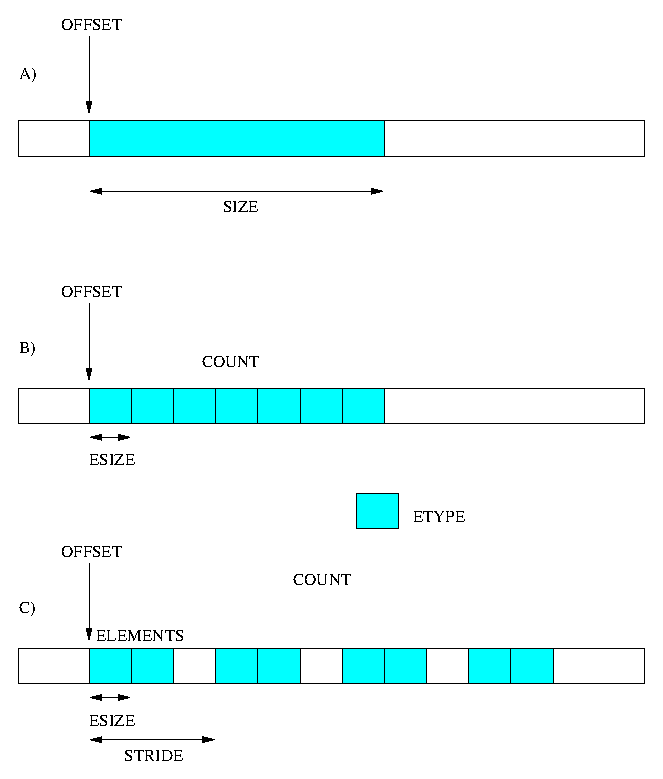
\includegraphics[scale=1.0]{figs_atoc.eps}

\subsection*{Single Contiguous Region Requests}

A single contiguous region is represented by a single structure.
The region can be specified as SIZE bytes at location OFFSET as
in figure A:

\begin{verbatim}
   PTYPE:
      offset = OFFSET
      num_ereqs = SIZE
      stride = 1
      num_blocks = 1
      ub = SIZE
      lb = 0
      aggregate_size = SIZE
      depth = 1
      num_contig_chunks = 1
      etype = PVFS_Request_byte
      stype = NULL
\end{verbatim}

Or can be specified as an array of COUNT integers as in figure B:

\begin{verbatim}
   PTYPE:
      offset = OFFSET
      num_ereqs = COUNT
      stride = 1
      num_blocks = 1
      ub = COUNT * 4
      lb = 0
      aggregate_size = COUNT * 4
      depth = 1
      num_contig_chunks = 1
      etype = PVFS_Request_int
      stype = NULL

   PVFS_Request_int:
      offset = 0
      num_ereqs = 4
      stride = 1
      num_blocks = 1
      ub = 4
      lb = 0
      aggregate_size = 4
      depth = 0
      num_contig_chunks = 1
      etype = NULL
      stype = NULL
\end{verbatim}

Note that default PVFS\_Request exist for standard data types including:
PVFS\_Request\_byte, PVFS\_Request\_char, PVFS\_Request\_short, PVFS\_Request\_int,
PVFS\_Request\_long, PVFS\_Request\_float, PVFS\_Request\_double.
Each of these standard types is defined with an etype of NULL which
indicates that the region is contiguous regardless of the other
parameters.

\subsection*{Strided Region Requests}

A data area made up of regular strided groups of contiguous elements
can also be represented with a single PINT\_Request structure.  A region
consisting of GROUPS groups of ELEMENTS items of type ETYPE with a size
of ESIZE each with a stride
between the first element of each group of STRIDE bytes would be as
in figure C:

\begin{verbatim}
   PTYPE:
      offset = OFFSET
      num_ereqs = ELEMENTS
      stride = STRIDE
      num_blocks = GROUPS
      ub = ((GROUPS - 1) * STRIDE) + (ELEMENTS * ESIZE)
      lb = 0
      aggregate_size = GROUPS * ELEMENTS * ESIZE 
      depth = 1
      num_contig_chunks = GROUPS
      etype = ETYPE
      stype = NULL
\end{verbatim}

Once again this assumes that ETYPE is a contiguous type.

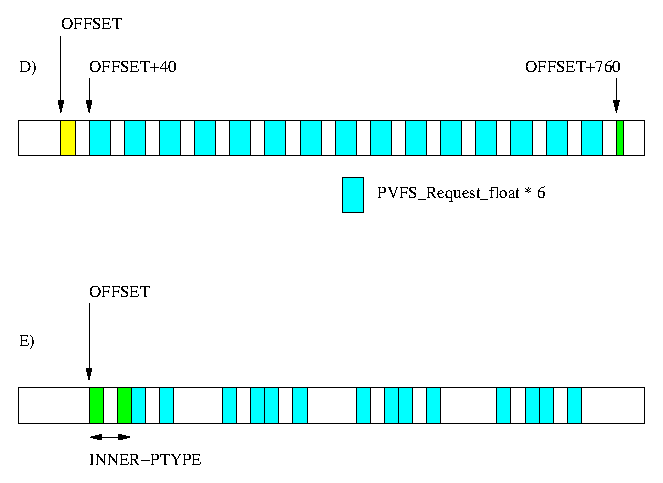
\includegraphics[scale=1.0]{figs_dtoe.eps}

\subsection*{Sequential Requests}

A data area may consist of a region that conforms to one type,
followed by a region that conforms to another.  Example might
include a strided region where one wants to begin and/or end
in the middle of a group, rather than have a integral number
of whole groups, or may be two unrelated segments of data.
For this, a sequence of PINT\_Request structures is specified
using the stype field to determine the sequence.  The offset
is specified relative to the beginning of the data area.

In this example we have a strided region shown in D.  We want to start
8 bytes into the first group (yellow), then have 15 whole groups (blue), and
finally end 4 bytes into the last group (green).  Each group is 6
elements, and each element is a float (4 bytes).  The stride
between groups is 48 bytes (12 floats).

\begin{verbatim}
   FIRST-PTYPE:
      offset = OFFSET
      num_ereqs = 4
      stride = 1
      num_blocks = 1
      ub = 764
      lb = 0
      aggregate_size = 380
      depth = 1
      num_contig_chunks = 17
      etype = PVFS_Request_float
      stype = NEXT-PTYPE
   
   NEXT-PTYPE:
      offset = OFFSET + 40
      num_ereqs = 6
      stride = 48
      num_blocks = 15
      ub = 764
      lb = 40
      aggregate_size = 364
      depth = 1
      num_contig_chunks = 16
      etype = PVFS_Request_float
      stype = LAST-PTYPE
   
   LAST-PTYPE:
      offset = OFFSET + 760
      num_ereqs = 1
      stride = 1
      num_blocks = 1
      ub = 764
      lb = 760
      aggregate_size = 4
      depth = 1
      num_contig_chunks = 1
      etype = PVFS_Request_float
      stype = NULL
\end{verbatim}

Note that ub, lb, aggregate\_size, depth, and num\_contig\_chunks always
refers to the region
represented down stream of the current PINT\_Request record, and not the
whole region, however ub and lb are still expressed in terms of the
entire data area.

\subsection*{Nested Types}

Any request can be built on top of another request.  When the base
request is
contiguous the result is as above, but when the base request is not
contiguous things are more complicated.  Examples include nested
strided regions and vectors of records that are only partially
accessed.

The following is a nested strided region.  There are 4 groups of
two "elements," with a stride of 8 elements.  Each element consts
of 2 groups of 6 integers (one element shown in green), with a stride
of 48 bytes.

\begin{verbatim}
   OUTER-PTYPE:
      offset = OFFSET
      num_ereqs = 2
      stride = 768
      num_blocks = 4
      ub = 3264
      lb = 0
      aggregate_size = 384
      depth = 2
      num_contig_chunks = 16
      etype = INNER-PTYPE
      stype = NULL

   INNER-PTYPE:
      offset = 0
      num_ereqs = 6
      stride = 48
      num_blocks = 2
      ub = 96
      lb = 0
      aggregate_size = 48
      depth = 1
      num_contig_chunks = 2
      etype = PVFS_Request_int
      stype = NULL
\end{verbatim}

Note that the offset, ub, and lb are in terms of the inner elements
and not of the entire buffer, thus the offset is the offset from the
beginning of that element to the first bit of data in that element.

\section{The PINT\_Request\_state}

When processing a request described with a PVFS\_Request the following
structures are used to keep track of how much of the request has been
processed.

\begin{verbatim}
   typedef struct PINT_reqstack {
      int32_t el;      /* number of element being processed */
      int32_t maxel;   /* total number of these elements to process */
      PINT_Request *rq;     /* pointer to request structure */
      PINT_Request *rqbase; /* pointer to first request is sequence chain */
      int32_t blk;     /* number of block being processed */
      PVFS_offset  chunk_offset; /* offset of beginning of current contiguous chunk */
   } PINT_reqstack;

   typedef struct PINT_Request_state {
      struct PINT_reqstack *cur; /* request element chain stack */
      int32_t lvl;        /* level in element chain */
      PVFS_size    bytes;      /* bytes in current contiguous chunk processed */
      PVFS_offset  buf_offset; /* byte offset in user buffer */
   } PINT_Request_state;
\end{verbatim}

The PINT\_Request\_state utilizes a stack to keep up with each level in the
element type chain.  For each level, a stack element records which block
and which element within the block is being processed as well as which
PVFS\_Request record in the sequence chain is being processed.  The
maxel and dtbase fields are used to reset each level each time it is
entered.  The PINT\_Request\_state records the level being processed
and a function used to process each contiguous block of data.  The bytes
field is used to record the results of a partial processing of bytes so
the processing can be paused and resumed later.

\section{PINT\_Process\_request interface}

Requests and distributions are processed using the interface described
here.  The caller allocates an array of SEGMAX offsets and an array of
SEGMAX segment sizes.  These are passed to the PINT\_Process\_request function
allong with an initialized PINT\_Request\_state, a PVFS\_Request, a
PVFS\_Request\_file\_data struct which includes distribution, distribution
parameters, metadata, and an EXTEND\_FLAG that indicates if the routine
should stop at the current end of file (if the value is zero) or should
extend the local file to the size needed to complete the request (if the
value is non-zero) in the even that the file ends before the end of the
request. A read will typically have a zero value and a write will
typically have a one value.  Other arguments to PINT\_Process\_request
include the maximum number of segments to process SEGMAX,
a maximum number of bytes to transfer BYTEMAX,
and a starting offset START\_OFFSET, and EOF\_FLAG argument returns
whether the end of the request is at or beyond the end of file.

\begin{verbatim}
   typedef struct PINT_Request_file_data {
      PVFS_size    fsize;     /* actual size of local storage object */
      int32_t server_nr;   /* ordinal number of THIS server for this file */
      int32_t server_ct; /* number of servers for this file */
      PVFS_Distribution *dist;
      PVFS_Dist_parm    *dparm;
      PVFS_boolean      extend_flag;
   } PINT_Request_file_data;
\end{verbatim}

PINT\_Process\_request fills in up to SEGMAX array entries, updates
SEGMAX to indicate the number of segments processed, updates BYTEMAX
to indicate the number of bytes processed, and updates START\_OFFSET and the
PINT\_Reqest\_state to indicate the last point in the request procssed.
The function attempts to process BYTEMAX bytes, but cannot process more
than SEGMAX contiguous regions.  The code is expected to be optimized
for the case where START\_OFFSET is equal to the value returned the last time
the function was called with the same PINT\_Request\_state.

\begin{verbatim}
   int PINT_Process_request(PINT_Request_state *req,
      PINT_Request_file_data *rfdata, int32_t *segmax,
      PVFS_offset *offset_array, PVFS_size *size_array,
      PVFS_offset *start_offset, PVFS_size *bytemax,
      PVFS_boolean *eof_flag, int mode);
\end{verbatim}

The MODE tells the request processor whether to process the
request in terms of the local file offsets on a server or local buffer
offsets on a client.  Clients should set this to PVFS\_CLIENT to
indicate that the data will be read into a contiguous buffer.  Servers
should set to PVFS\_SERVER to indicate that the offsets computed by the
distribution module should be used as the local file offsets.
A third mode PVFS\_CKSIZE indicates that the routine should count how
many bytes up to BYTEMAX are left in the request, but does not alter the
requset state or update the SIZE\_ARRAY or OFFSET\_ARRAY.

Before calling PINT\_Process\_request for a given request for the first
time, the caller needs to allocate a PINT\_Request\_state structure.
This is done by calling PINT\_New\_request passing in a pointer to the
request.  Theoretically multiple request states can exist for the same
request, thought there is really no need to do such a thing.

\begin{verbatim}
struct PINT_Request_state *PINT_New_request_state (PINT_Request *request);
\end{verbatim}

The new request state is positioned at the beginning of the request.
The caller must also allocate a 64-bit start\_offset, as well as
the offset and size arrays, eof\_flag, segmax, and bytemax.  Each time
PINT\_Process\_request is called, the segmax, bytemax, and eof\_flag
should be reset to the proper values, as the function returns results in
these variables as well as taking inputs from them.  The offset and size
arrays are overwritten each time PINT\_Process\_state is called.  The
start\_offset variable is normally NOT reset between calls as the
caller normally wishes to continue translating the request from the
point left off previously.  After completing the processing of the
request, the caller is also responsible for freeing the request state
structure with a call to PINT\_Free\_request.

\begin{verbatim}
void PINT_Free_request_state (PINT_Request_state *req);
\end{verbatim}

The following is a sample of code calling the request processing
routines.  It processes an entire request using no more than SEGMAX
contiguous sements at a time and no more than BYTEMAX bytes at a time.

\begin{verbatim}
#include <pvfs-types.h>
#include <pint_distribution.h>

#define SEGMAX 32
#define BYTEMAX 250

do_a_request(PINT_Request *req,
      PVFS_Distribution *dist,
      PVFS_Dist_parm *dparm,
      PVFS_Meta meta)
{
   int i;

   // PVFS_Process_request arguments
   PINT_Request_state *reqs;
	PINT_Request_file_data rfdata;
   PVFS_offset offset_array[SEGMAX];
   PVFS_size size_array[SEGMAX];
   PVFS_offset offset;
   PVFS_size bytemax;
   int32_t segmax;
   PVFS_boolean extend_flag;
   PVFS_boolean eof_flag;

   reqs = PINT_New_request_state(req);
   rfdata.server_nr = 0;
   rfdata.server_ct = 1;
   rfdata.fsize = 10000000;
   rfdata.dist = dist
   rfdata.dparm = dparm
   rfdata.extend_flag = 0;
   eof_flag = 0;
   offset = 0;
   do {
      segmax = SEGMAX;
      bytemax = BYTEMAX;
      PINT_Process_request(reqs, &rfdata, &segmax, offset_array,
            size_array, &offset, &bytemax, &eof_flag, PINT_SERVER);
      printf("processed %lld bytes in %d segments\n", bytemax, segmax);
      for (i = 0; i < segmax; i++)
      {
         printf("segment %d: offset=%lld size=%lld\n", i,
               offset_array[i], size_array[i]);
      }
   } while (offset != -1);
}
\end{verbatim}


\end{document}







